%
% section 6.1.2
%
\subsection{Οργάνωση DNS}

Η ιεραρχία του χώρου ονομάτων είναι αντίστοιχη με την ιεραρχία των εξυπηρετητών (σχήμα \ref{6-3})

\begin{figure}[!ht]
  \centering
  \includegraphics[width=0.85\textwidth]{images/chapter6/6-3}
  \caption {\textsl{Ιεραρχία Εξυπηρετητών DNS}}
  \label{6-3}
\end{figure}

Κάθε εξυπηρετητής είναι υπεύθυνος για ένα τμήμα του χώρου ονομάτων που ονομάζεται \emph{ζώνη (zone)}.

\begin{inthebox}
\textbf{Μα αν ένας εξυπηρετητής είναι υπεύθυνος για μια περιοχή (domain) αυτό δεν σημαίνει ότι η ζώνη περιέχει όλα τα μηχανήματα της περιοχής; Ποια είναι η διαφορά μεταξύ ζώνης και περιοχής;}

Η ζώνη περιέχεται σε ένα αρχείο μέσα στον εξυπηρετητή και περιέχει εγγραφές με διευθύνσεις και ονόματα. Αν έχουμε μια περιοχή που δεν περιέχει άλλες υποπεριοχές αλλά μόνο μηχανήματα, το αρχείο ζώνης μπορεί πράγματι να περιέχει όλα τα μηχανήματα της περιοχής. Για παράδειγμα η περιοχή freebsdworld.gr δεν περιέχει άλλες υποπεριοχές αλλά μόνο μηχανήματα (hosts). Δείτε παρακάτω ένα απόσπασμα της αντίστοιχης ζώνης:

\begin{verbatim}
ns1             IN      A       193.183.99.68
ns2             IN      A       46.19.141.199
equinox         IN      A       193.183.99.68
falcon          IN      A       46.19.141.199
\end{verbatim}

(Οι εγγραφές τύπου ``Α'' υποδηλώνουν μηχανήματα (hosts))

Ας πάρουμε όμως την περίπτωση μια περιοχή να περιέχει υποπεριοχές. Δείτε για παράδειγμα το σχήμα \ref{6-12}. 

\begin{figure}[!ht]
  \centering
  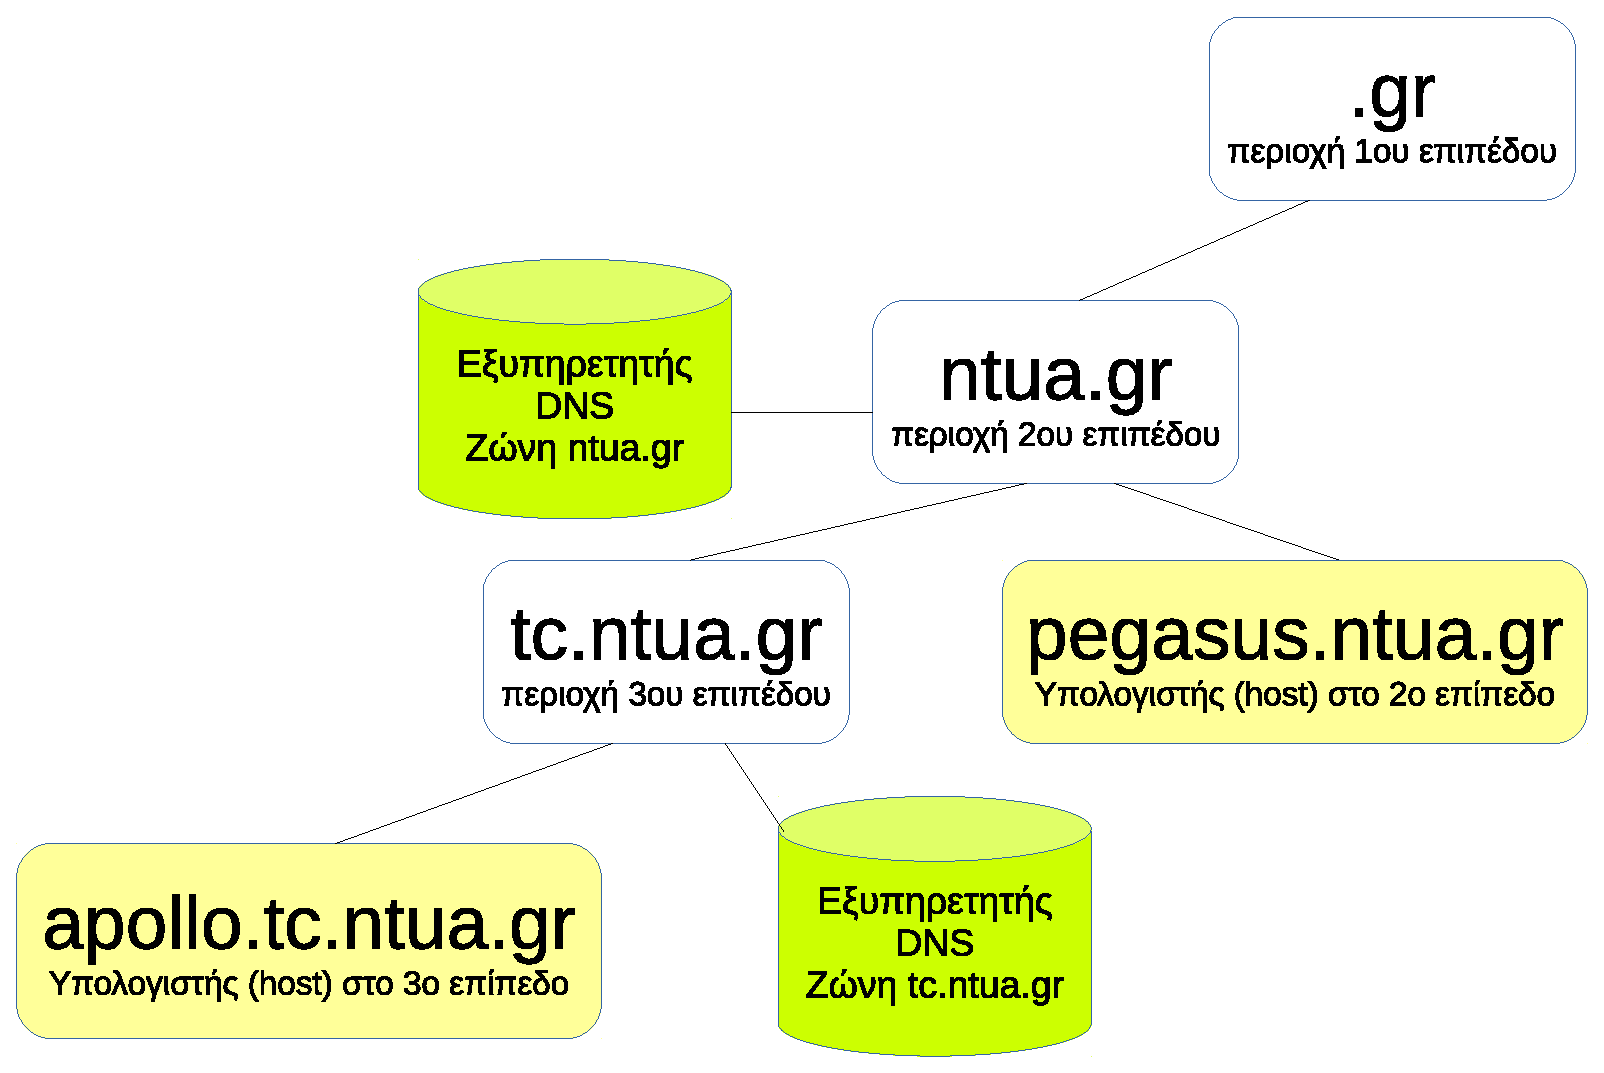
\includegraphics[width=0.95\textwidth]{images/chapter6/6-12}
  \caption {\textsl{Περιοχές και Ζώνες}}
  \label{6-12}
\end{figure}

Υπάρχει εδώ η περιοχή \textbf{ntua.gr} (στο 2ο επίπεδο) και η \textbf{tc.ntua.gr} (στο 3ο επίπεδο). Σε κάθε επίπεδο υπάρχει από ένας υπολογιστής (host) και ένας εξυπηρετητής DNS.

Τι περιέχει η ζώνη \textbf{ntua.gr} στο DNS 2ου επιπέδου; Περιέχει μια εγγραφή για τον υπολογιστή \textbf{pegasus.ntua.gr} που είναι στο ίδιο επίπεδο, αλλά \textbf{δεν} περιέχει για τον \textbf{apollo.tc.ntua.gr} που είναι στο 3ο επίπεδο!

Αντί για αυτό, η ζώνη δευτέρου επιπέδου διαθέτει μια εγγραφή που δείχνει στην IP του εξυπηρετητή DNS 3ου επιπέδου και ορίζει ότι αυτός είναι υπεύθυνος για την υποπεριοχή \textbf{tc.ntua.gr}. Αν ο DNS 2ου επιπέδου δεχθεί ένα ερώτημα του τύπου ``ποια είναι η διεύθυνση του υπολογιστή apollo.tc.ntua.gr'' μπορεί:

\begin{itemize}
\item Είτε να ρωτήσει τον εξυπηρετητή DNS 3ου επιπέδου (τον οποίο γνωρίζει καθώς η διεύθυνση του περιέχεται στη δική του ζώνη)
\item Είτε να παραπέμψει όποιον έθεσε το ερώτημα στον εξυπηρετητή DNS 3ου επιπέδου στέλνοντας του μια απάντηση του τύπου ``υπεύθυνος για την υποπεριοχή είναι ο εξυπηρετητής DNS με IP x.x.x.x''
\end{itemize}

Είναι όμως φανερό από τα παραπάνω ότι η ζώνη που περιέχεται στον εξυπηρετητή DNS 2ου επιπέδου δεν περιέχει τις πληροφορίες όλης της περιοχής \textbf{ntua.gr}. Γενικά μια ζώνη περιέχει συνήθως πληροφορίες για ένα μόνο τμήμα ενός χώρου ονομάτων και τα υπόλοιπα τμήματα της περιοχής μπορεί να είναι αποθηκευμένα σε άλλες ζώνες και εξυπηρετητές.\\
\end{inthebox}

\begin{figure}[!ht]
  \centering
  \includegraphics[width=0.95\textwidth]{images/chapter6/6-4}
  \caption {\textsl{Οργάνωση σε Ζώνες}}
  \label{6-4}
\end{figure}

Τελικά, για να βρεθεί μια αντιστοίχιση μπορεί να χρειαστεί να ερωτηθούν αρκετοί εξυπηρετητές.

Για κάθε ζώνη πρέπει να υπάρχει ένας κύριος (primary) και ένας δευτερεύον (secondary) εξυπηρετητής. O δευτερεύων κρατάει αντίγραφα των δεδομένων του κύριου εξυπηρετητή. Η βάση δεδομένων μπορεί να ενημερωθεί δυναμικά προσθέτοντας, διαγράφοντας ή τροποποιώντας τις εγγραφές της. Για να προστεθεί ένα μηχάνημα (host) σε μια ζώνη ο διαχειριστής προσθέτει τις αντίστοιχες πληροφορίες (όνομα και διεύθυνση) στο αντίστοιχο αρχείο ζώνης. Ο δευτερεύων εξυπηρετητής συνήθως ενημερώνεται αυτόματα για την αλλαγή μέσω του κύριου.

Σχεδόν κάθε οργανισμός, εταιρεία, πανεπιστήμιο κλπ διαθέτει ένα τοπικό εξυπηρετητή ονομάτων που είναι γνωστός και ως \emph{επιλεγμένος ή προεπιλεγμένος (default)} εξυπηρετητής. Ο εξυπηρετητής αυτός μπορεί να απαντήσει σε ερωτήματα για τα ονόματα και τις διευθύνσεις των μηχανημάτων του τοπικού (εσωτερικού) δικτύου (διαθέτει τις απαραίτητες ζώνες) αλλά απαντάει και για ερωτήματα που αναφέρονται σε υπολογιστές και διευθύνσεις εκτός της εταιρίας (στο Διαδίκτυο). Για το σκοπό αυτό ρωτά άλλους εξυπηρετητές και μπορεί αν χρειαστεί να φτάσει και μέχρι τους εξυπηρετητές ρίζας (Για λόγους απόδοσης μπορεί φυσικά να αποθηκεύει προσωρινά τα αποτελέσματα).

Το \textbf{πρωτόκολλο DNS} βρίσκεται στο επίπεδο εφαρμογής και χρησιμοποιεί το μοντέλο πελάτη -- εξυπηρετητή. Ο πελάτης ονομάζεται \emph{αναλυτής (resolver)}. Το πρωτόκολλο DNS υποστηρίζει τη μετατροπή ονομάτων σε διευθύνσεις και το ανάστροφο (ανάλυση ή resolution) καθώς και την ενημέρωση δεδομένων μεταξύ των εξυπηρετητών ονομάτων.

Η \textbf{ανάλυση ονομάτων (name resolution)} είναι η διαδικασία με την οποία αναλυτές και εξυπηρετητές DNS συνεργάζονται για να βρουν δεδομένα εντός του χώρου ονομάτων. Για την ανεύρεση δεδομένων οι εξυπηρετητές DNS χρειάζονται μόνο τις διευθύνσεις IP των εξυπηρετητών κορυφής (ρίζας). Οι εξυπηρετητές ρίζας γνωρίζουν όλες τις περιοχές ανωτάτου επιπέδου και μπορούν να υποδείξουν τους εξυπηρετητές περιοχών με τους οποίους μπορεί να γίνει επαφή.